\documentclass[12pt, a4paper]{article}

\usepackage[utf8]{inputenc}
\usepackage[T1]{fontenc}
\usepackage{lmodern}

\usepackage[spanish]{babel}

\usepackage{amsmath,amssymb}

\usepackage{booktabs}
\usepackage{longtable}
\usepackage{array}

\usepackage{geometry}
\geometry{left = 2.5cm, right = 2.5cm, top = 2.5cm, bottom = 2.5cm}

\usepackage{graphicx, subfig}

\usepackage{hyperref}
\hypersetup{
    colorlinks=true,
    linkcolor=blue,
    filecolor=magenta,
    urlcolor=cyan,
}

\usepackage{xcolor}
\usepackage{caption}
\captionsetup[table]{font = small, skip = 5pt}

\usepackage{indentfirst}

\usepackage{setspace}

\usepackage{fancyhdr}

\pagestyle{fancy}
\fancyhf{}

\fancypagestyle{plain}{
    \fancyhf{}
    \fancyfoot[C]{Página~\thepage}
    \renewcommand{\headrulewidth}{0pt}
    \renewcommand{\footrulewidth}{1pt}
}

\fancyhead[L]{\textit{Título}}
\fancyhead[R]{\textit{Orozco, Pizarro}}

\fancyfoot[C]{Página~\thepage}

\renewcommand{\headrulewidth}{1pt}
\renewcommand{\footrulewidth}{1pt}

\title{Trabajo Práctico N°1}
\author{Orozco Lopez Alejandro, Pizarro Dal Maso Federico}
\date{8 de Septiembre, 2025}

\begin{document}

\setlength{\parskip}{1em}

\captionsetup[table]{name=Tabla}

\maketitle

\begin{abstract}
    
Abstract

\end{abstract}

\section{Introducción}

Actualmente la compresión de imágenes es una técnica con múltiples aplicaciones. 
Las imágenes están tomando un papel fundamental en la comunicación global. 
Una de las principales por las que una compresión de imágenes eficaz es crucial es su capacidad de reducir el espacio de almacenamiento necesario para estos archivos.

Para ello, trabajaremos con el Análisis de Componentes Principales (PCA). 
Este método nos ayuda a comprimir por medio de la reducción de dimensionalidad.
Transforma los datos en un nuevo sistema de coordenadas, donde el primer eje (componente principal) captura la mayor varianza de los datos, seguido de los ejes subsiguientes que capturan varianzas decrecientes.

En otras palabras, imaginemos una imagen como una gran matriz donde algunas columnas pueden tener dependencias lineales. 
La correlación entre píxeles puede transformarse en un nuevo conjunto de variables no correlacionadas, llamadas componentes principales. 
Ellos capturan la información esencial de la imagen, reduciendo la redundancia y permitiendo una compresión eficiente.

El objetivo es implementar compresión por bloques usando PCA, reconstruir las imágenes a partir de las componentes conservadas y evaluar la calidad mediante métricas como el error cuadrático medio (MSE) y la fracción de energía conservada. 
También se analizará la relación entre el grado de compresión y la pérdida visual.

\section{Ejercicio 1}

El propósito del primer ejercicio fue analizar la correlación entre los píxeles vecinos verticalmente y comprobar como una transformación basada en PCA puede desacoplar las dos variables con el objetivo de facilitar la compresión.

A cada imagen la cargamos en escala de grises y la normalizamos.
Formamos vectores de tamaño $2\times 1$ con pixeles contiguos verticales: \(X = \begin{bmatrix} X_1 \\ X_2 \end{bmatrix}\). 
Graficamos la dispersión de $X_1$ vs $X_2$ junto con la imagen original. Estimamos el coeficiente de correlación de Pearson
    \[
      r = \frac{\operatorname{cov}(X_1,X_2)}{\sigma_{X_1}\sigma_{X_2}},
    \]
el cual cuantifica la dependencia lineal entre píxeles vecinos.
Para descorrelacionar aplicamos PCA: centramos los datos, calculamos la matriz de covarianza $C_X$, hicimos la descomposición en autovalores/autovectores y proyectamos los datos sobre los autovectores.
    \[
      Y = E^\top (X - \mu),
    \]
donde $E$ son los autovectores de $C_X$ y $\mu$ la media.

Los gráficos obtenidos son los siguientes:

\begin{figure}[htbp]
  \centering
  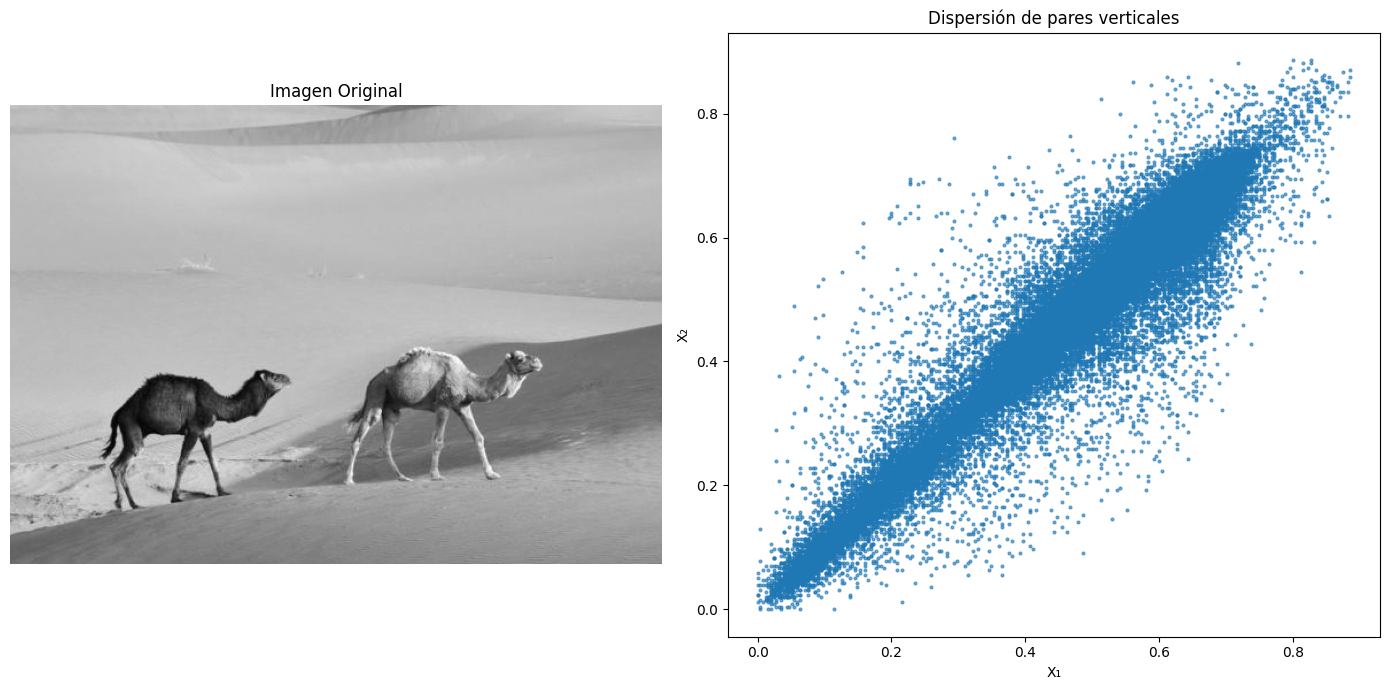
\includegraphics[width=0.8\textwidth]{img1a1.png}
  \caption{img\_01 (escala de grises).}
  \label{fig:img01}
\end{figure}

\begin{figure}[htbp]
  \centering
  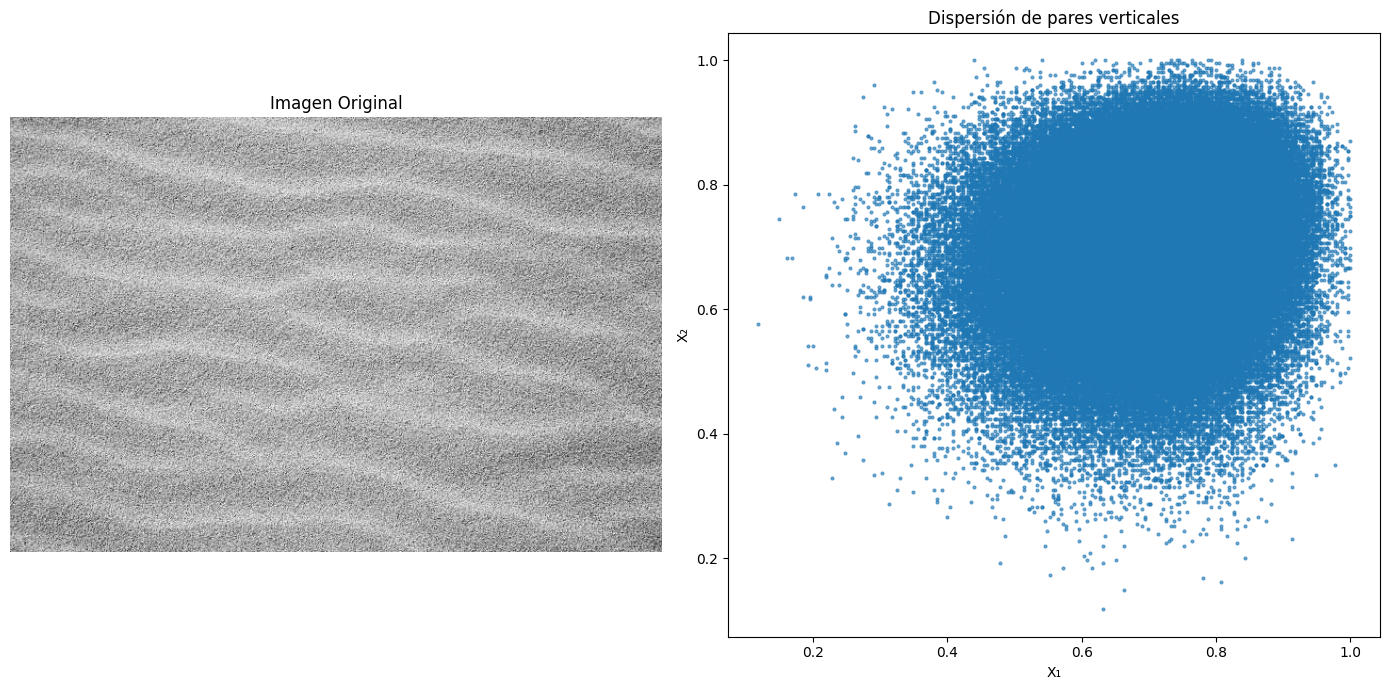
\includegraphics[width=0.8\textwidth]{img1a2.png}
  \caption{img\_01 (escala de grises).}
  \label{fig:img02}
\end{figure}

\begin{figure}[htbp]
  \centering
  \subfloat[img\_01]{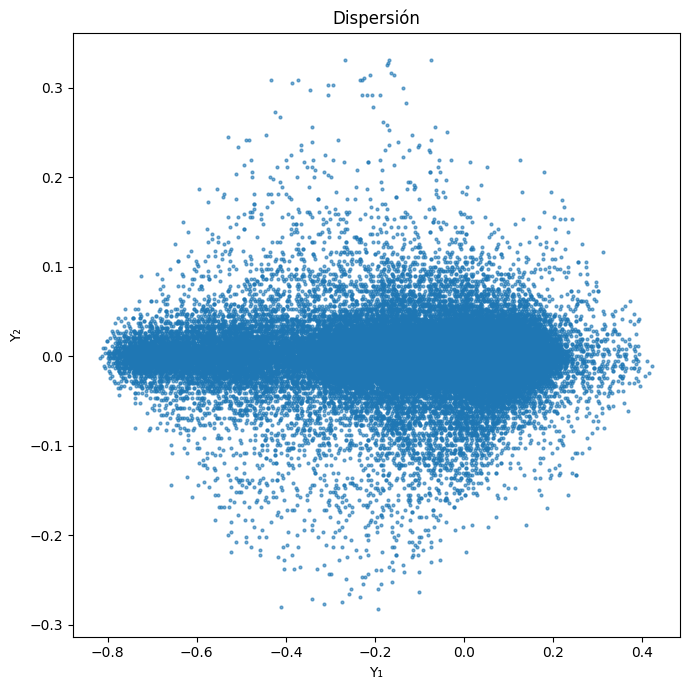
\includegraphics[width=0.48\textwidth]{img1c1.png}\label{fig:img03}}
  \hfill
  \subfloat[img\_02]{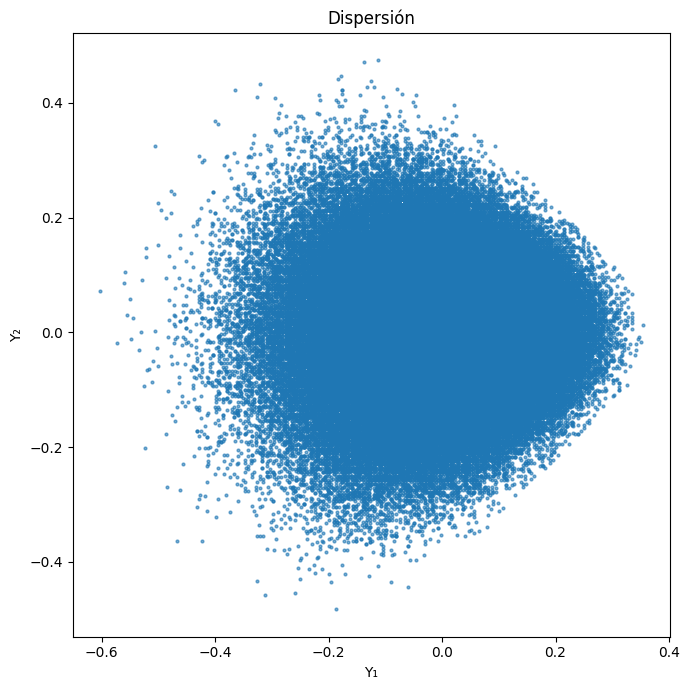
\includegraphics[width=0.48\textwidth]{img1c2.png}\label{fig:img04}}
  \caption{Gráficos de dispersión de la transformación.}
  \label{fig:imgs_comp}
\end{figure}

\section{Ejercicio 2}

\section{Ejercicio 3}

\section{Ejercicio 4}

\end{document}